%!TEX root = ../paper.tex

%%%%%%%%%%%%%%%%%%%%%%
\section{The Outcomes of Code Reviews} \label{sec:outcomes}
%%%%%%%%%%%%%%%%%%%%%%

\begin{figure}[t] %  figure placement: here, top, bottom, or page
   \centering
   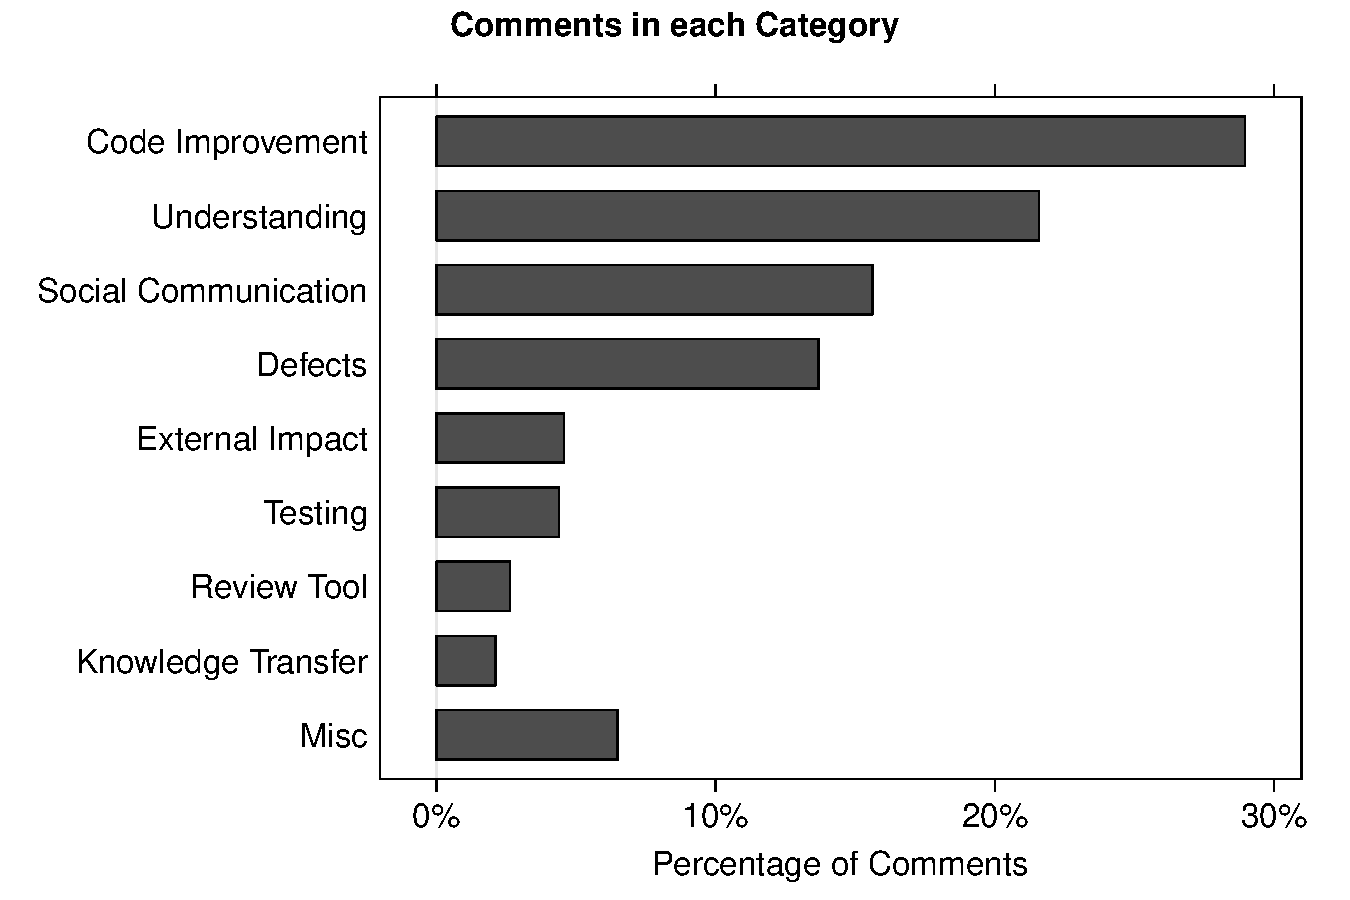
\includegraphics[width=\columnwidth]{comments.pdf}
   \vspace{-1.5em}
   \caption{Proportion of comments by card sort category.}
   \label{fig:comments}
   \vspace{-1.5em}
\end{figure}

Our second research question seeks to understand what the actual outcomes of code reviews are, and whether they match the motivations and expectations outlined in the previous section. To that end, we conducted indirect field research~\cite{lethbridge2005studying} by analyzing the content of 200 threads (corresponding to 570 comments) recorded by CodeFlow. \figref{fig:comments} shows the categories of comments found through the card sort.

\textbf{Code Improvements:} The most frequent category, with 165~(29\%) comments, is \emph{code improvements}. In detail, among \emph{code improvements} comments we find 58 on using better code practices, 55 on removing not necessary or unused code, and 52 on improving code readability.

\textbf{Defect Finding:} Although \emph{defect finding} is the top motivation and expected outcome of code review for many practitioners, the category \emph{defect} is the only the fourth most frequent, out of nine items, with 78 (14\%) comments. Among \emph{defect} comments, 65 are on logical issues (\eg a wrong expression in an if clause), 6 on high-level issues, 5 on security, and 3 on wrong exception handling.

\textbf{Knowledge Transfer:} Concerning the other expected outcomes of code reviews, we did not expect to find evidence about them, because of their more ``social''--thus harder to quantify—nature. Nevertheless, we found some (12) comments specifically about \emph{knowledge transfer}, where the reviewers were directing the code change author to external resources (\eg internal documentation or websites) for learning how to tackle some issues. This provides additional evidence on the importance of this aspect of reviews.

\subsection{Finding Defects: When Expectations Do Not Meet Reality}

Why do we see this significant gap in frequency between \emph{code improvements} and \emph{defects} comments? Possible reasons may be that our sample of 570 comments is too small to represent the population, that the submitted changes might require less need fixing of ``real'' defects than of small code improvements, or that programmers could consider \emph{code improvements} as actual defects. However, by triangulating these numbers with the interview discussions, the survey answers, and the other categories of comments, another reason seems to justify this situation. First, we start by noting that most of the comments on \emph{defects} regard uncomplicated logical errors, \eg corner cases, common configuration values, or operator precedence. Then, from interview data, we see that: \begin{inparaenum}[(1)]
\item most interviewees explained how, with tool-based code reviews, most of the found defects regard \quotation{logic issues--where the author might not have considered a particular or corner case}; 
\item some interviewees complained that the quality of code reviews is low, because reviewers only look for easy errors: \quotation{{\normalfont [Some reviewers]} focus on formatting mistakes because they are easy {\normalfont [...]}, but it doesn't really help. {\normalfont [...]} In some ways it's kind of embarrassing if someone asks you to do a code review and all you can find are formatting mistakes when there are real mistakes to be found}; and 
\item other interviewees admitted that if the code is not among their codebase, they look at \quotation{obvious bugs (such as, exception handling).} Finally, managers mentioned \quotation{catching early obvious bugs} or \quotation{finding obvious inefficiencies or errors} as reasons for doing code review.
\end{inparaenum}
These points illustrate that the reason for the gap between the number of comments on \emph{code improvements} and on \emph{defects} is not to be found in problems in the sample or in classification misconceptions, but it is rather just additional corroborating evidence that the outcome of code review does not match the main expectation of both programmers and managers—finding defects. Review comments about defects are few, comprising one-eighth of the total in our sample, and mostly address ``micro'' level and superficial concerns; while programmers and managers would expect more insightful remarks on conceptual and design level issues. Why does this happen? The high frequency of understanding comments hints at the answer to our question, addressed in the next section.
